\setchapterpreamble[u]{\margintoc}
\chapter{Approach}
\labch{Approach}

\section{Motivation}
\labsec{Motivation}

The basic approach of this work can be split into two steps:
\begin{enumerate}
    \item A differentiable renderer which can generate images of brush strokes from a parameter representation.
    \item An optimization procedure that iteratively approximates an image through brush strokes representations.
\end{enumerate}

The two step approach can be motivated by comparing the optimization procedure to the
actual process of painting an image.
An artist will most likely not pick single color particles to then place them on
the canvas.
Instead, the artist uses a brush or other utilities (see Pollock or others) to place
more paint with a single action.
\todo{image that shows different types of paint and tools etc.}
This of course limits the control over each individual drop of paint but maintains
enough control to still create very delicate details in paintings.
This trade-off varies for different brush sizes and for this reason an artist must
choose the brush size depending on the content.

An example would be the painting of a uniformly colored sky.
By using a large brush size the artist can cover a lot of canvas in relatively little
time as well as keep the color well distributed over the canvas because the brush
will spread color more or less evenly over its footprint.
On the other hand, if one were to draw a sky with the smallest brush available,
not only would it take forever to paint, it would also be hard to keep the paint
evenly distributed over multiple strokes.

Now, translating this onto the given problem of recreating/approximating an image
through brush strokes, it would mean to limit the process to only use what we would
describe as brush strokes. \todo{reformualte this}

An equivalent example would be the game of Tangram.

\begin{marginfigure}
    \includegraphics{tangram}
    \caption[]{An Example of Tangram.}
    \labfig{tangram}
\end{marginfigure}

Tangram is a Chinese puzzle game that has the objective of replicating a given silhouette
only with a set of 7 unique shapes.
The shapes may not overlay or be cut or anything.
Quite similarly, the objective for an optimizer is to replicate an image by only
using brush strokes.

\begin{marginfigure}
    \includegraphics{genetic_starry_night}
    \caption[]{Starry Night approximated by a genetic algorithm using only circles. \url{https://effyfan.com/2018/03/02/w6-van-gogh-flowfield/}}
    \labfig{genetic}
\end{marginfigure}


This is a similar task to what genetic algorithms already can do and have done in
order to approximate images by other geometric shapes or even smaller photos (also 
known as the popular photo mosaic effect).
\paragraph{Genetic algorithms} follow a random sampling approach that 'evolves' like genomes do.
Basically starting with a random set of circles that are parameterized by their position,
radius and color; it then chooses the most successful samples and resamples again
in a region around these.
This process is repeated again and again, until a certain level of convergence is reached.

\begin{figure}
    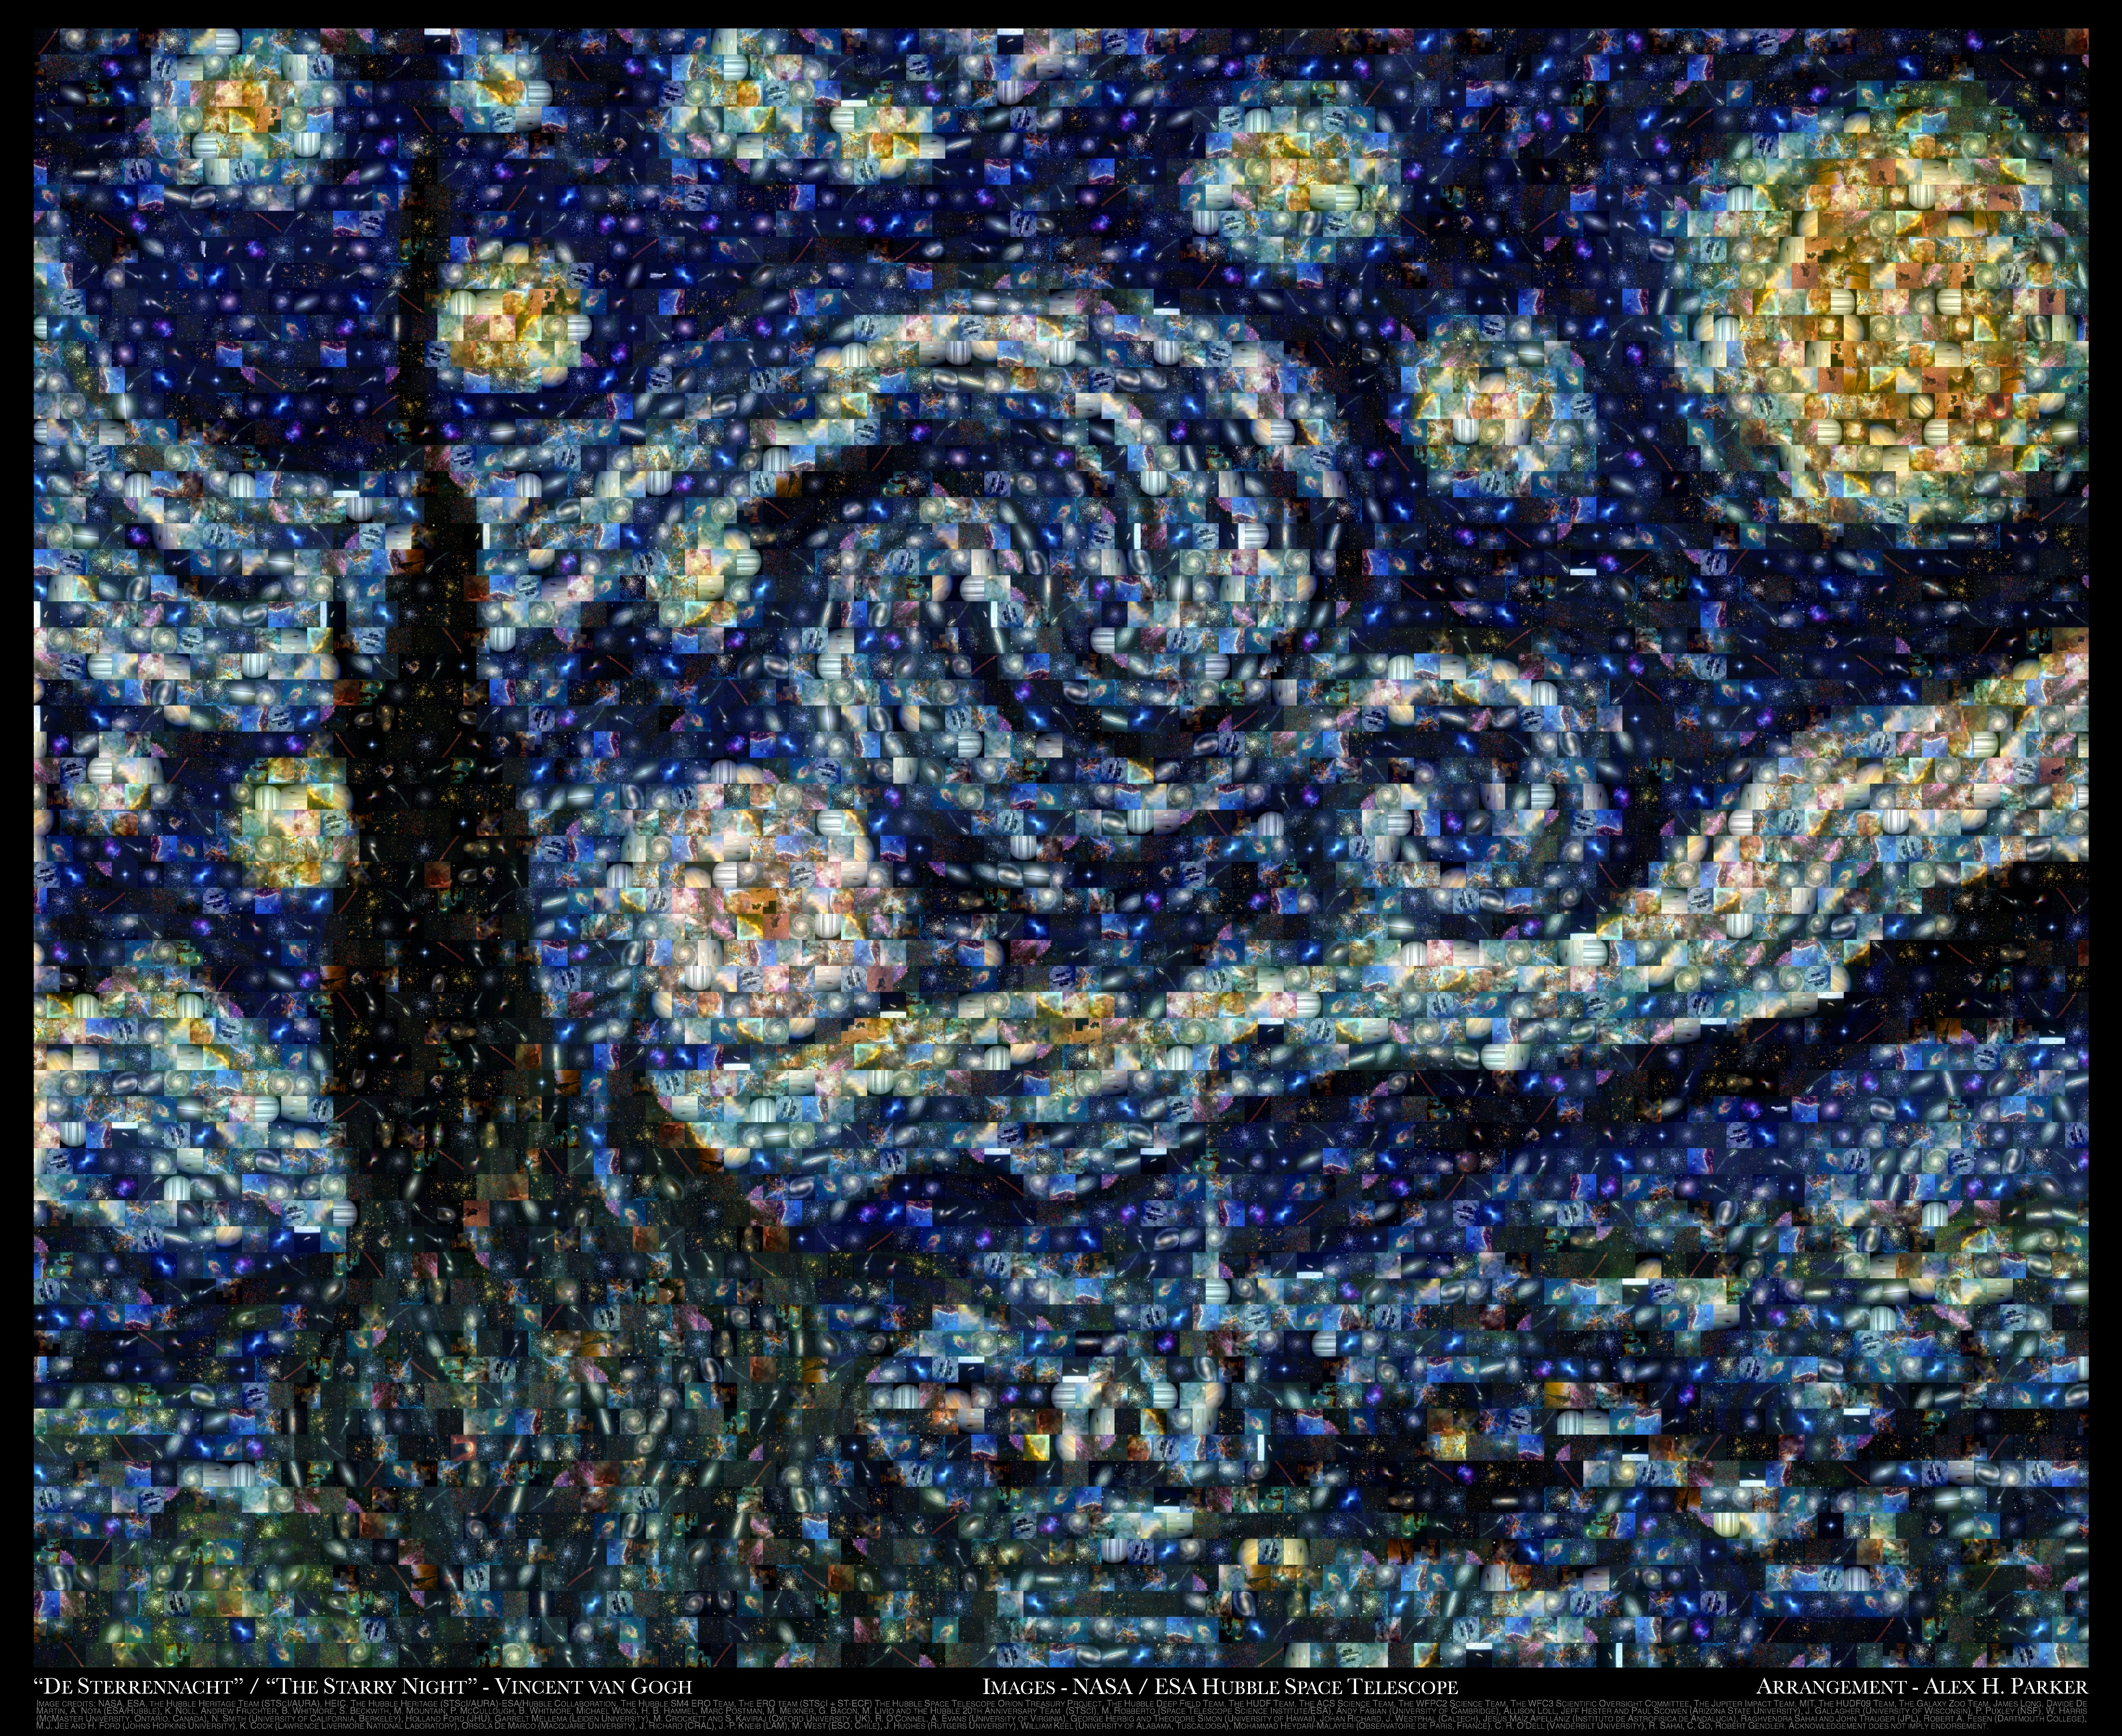
\includegraphics{photomosaic_starry_night}
    \caption[]{Photo mosaic of Starry Night using only images by the Hubble Space Telescope. \url{http://www.astro.uvic.ca/~alexhp/new/figures/starrynight_HST.001.jpg}}
    \labfig{photomosaic}
\end{figure}


As well as this does work, it is very much computationally expensive as most samples
will not fit the image, thus searching for the tiny set fitting shapes requires
to evaluate all the bad shapes as well.
Since brush strokes have many more degrees of freedom and artworks usually consist
of upwards of a few thousand brush strokes this will not be applicable to this problem
until computational resources have become a few magnitudes more powerful.

This premise can be overcome, though, by using something that is known as as a differentiable
renderer.
\paragraph{Differentiable renderers} allow for the previously described task to be
feasible as random sampling is replaced by gradient descent.
A differentiable renderer is capable of creating shapes in the pixel domain by only
using differentiable operations.
Ordinary renderers do not have this property as they rely on faster operations that are
not differentiable as most renderers are not used in this context.
Also, creating a differentiable pipeline to render a circle from the tuple (position,
 radius, color) is a much harder task than calculation the shape of a circle beforehand
and then projecting the shape onto the pixels in an image and coloring them accordingly.
Nonetheless it is theoretically possible to create such a renderer.

Going back to the task of rendering brush strokes, it would be even harder to think
of a pipeline that uses only differentiable functions and is able to draw brush strokes
of a reasonable quality from a set of parameters.

This is where neural networks give an opportunity to avoid this problem.
Neural network are inherently differentiable and previous works have shown that
they are capable of high resolution and high quality conditional image generation.
One could easily think of a generator setup that takes as an input the parameters of
a brush stroke as well as some noise and then outputs an image of the according
brush stroke with possibly some variability in outline shape or other characteristics.

This principle was proposed by \cite{japanese neural renderer} as it facilitates
training of reinforcement learning based networks.

Inspired by this, the approach becomes more clear.
First, a differentiable renderer in form of a neural network is trained.
Then this renderer is used by an optimization procedure that uses gradient descent
to approximate an artwork as a input parameters batch of the renderer.

Both steps require some tricks to avoid pitfalls like computational limitation which
are outlined in the following two sections.

\section{Neural Renderer}
\labsec{NeuralRend}

The neural renderer is inspired by previous works (\todo{cite these works}) and 
is required to be differentiable and should be based on a rather simple architecture.
Especially since complicated architectures impose computational burdens and could
possibly distort the gradients for optimization.

\subsection{Data Set}
\labsubsec{dataset}

Unfortunately there is no data set available for this task which means that the data set
must be specifically created for this approach.

There are several sources for brush strokes that are evaluated in the following part.


\subsubbsection{Brush Stroke Images}
\labsubsubsec{bsimages}

There are multiple sets of handrawn brush strokes available online.
Most notably there is a set of various well classified colors and brush styles created
by 'zolee' \todo{reference this} on the plattform \url{onlygfx.com}.
It cosists of approximately 1000 brush strokes that mostly follow rather straight
horizontal paths.
Brush strokes are mostly grouped by color and painting technique (oil, acrylic, watercolor...).
All images are in the PNG format and the area around the brush stroke was made 
transparent in a post-editing step.

This data set has the advantage that it consists of real world brush strokes that
were painted under presumably reproducible conditions.
On the other side, brush strokes are of mostly the same width throughout the data set
and also do not come with information which path the brush took or any other non-visual
information.
Also, the data is very sparse.
Many color shades are not represented which means that the generator would have to
'guess' them or simply would not be capable of rendering any brush strokes in this color.

It seems that this data set would be nice to replicate real world brush strokes
as images but limitations to the data make it unlikely that a generator could learn
a coherent representation from this.

\subsubbsection{Painting Libraries}
\labsubsubsec{libmypaint}

The mentioned work of SPIRAL \todo{cite this} relies on opposite data to real world
images.
They used the painting library 'libmypaint' \cite{libmypaint} to generate brush strokes
from parameters in real time during training.

The obvious advantage of this and other painting libraries is the fact that one
can fully control the output through parameters.
This makes it much easier as the whole space of input parameters for the renderer
can be covered and avoids pitfalls like they were described in \ref{bsimages}.

Still, this data set falls short regarding the authenticity of rendered strokes.
Especially the inner area of the stroke shows a uniform color which is far from
what real brush strokes would look like.

This data set is better suited for our task than the given images are but will tend
to make all rendering look a bit 'cartoonish' or flat, which could in turn limit
convergence during the latter optimization process.

\subsubbsection{Fluid Simulation}
\labsubsubsec{fluidpaint}

Fluid Paint \todo{cite website} is a project by \todo{name this guy} that uses simple
fluid dynamics to give artificial brush strokes a more plastic look.
It is implemented in JavaScript and OpenGL \todo{reference both}.

There is a C++ based version in the repository of SPIRAL which is also fitted with
python bindings by \todo{name that guy}.

Using these python bindings, it possible to generate brush strokes locally outside
of a web browser.

The quality and controllability of fluid paint falls right in between the two previously
mentioned datasets.
The generated brush strokes look distinctively better than those generated with 'libmypaint'
but still lack the quality of the real world images.
Concerning controllability, FluidPaint allows to control the path of the brush stroke
handle rather than the brush stroke itself.
This is a vast improvement over the images of 'zolee' but induces some offsets to
a given path as opposed to 'libmypaint'.

It seems that this is reasonable compromise between the previously mentioned data sets.
Although real time data generation in not possible with the library, it can be parallelized
to allow for the creation of large data sets in a reasonable time frame.

Even though this data set still has some weaknesses, it comes in as the probably best
choice for training a differentiable renderer because of the noted reasons.

Other notable mentions are the painting programs \todo{these two weird software stuff things}
which allow for even more authentic brush strokes but lack a well documented interface
in order to generate a vast number of brush strokes.


\subsubbsection{Brush Stroke Formalism}
\labsubsubsec{formalism}
With the means of data set production seized \todo{cut this joke}, what is left
is to formulate the parameter that define the brush strokes.


\subsection{Architecture}
\labsubsec{arch}

\subsection{Training}
\labsubsec{train}

\subsection{Results}
\labsubsec{results}

\section{Stroke Approximation}
\labsec{StrokeApprox}

\subsection{Dataset}
\labsubsec{dataset}

\subsection{Image Composition}
\labsubsec{composition}

\subsection{Optimization}
\labsubsec{opt}

\subsection{Results}
\labsubsec{results}

